\documentclass[11pt,report]{jsbook}
\usepackage[dvipdfmx]{color}
\usepackage[dvipdfmx]{graphicx}
\usepackage{ascmac}
\usepackage{wrapfig}
\usepackage{titlesec}
\usepackage{picture}
\usepackage[usenames]{color}
\usepackage{okumacro}
\usepackage[Bjornstrup]{fncychap}
%\usepackage[usenames,divpsnames]{xcolor}                                                                                                                                                                                                                                                                                                                              

%colors                                                                                                                                                                                                                                                                                                                                                               
\definecolor{teal}{RGB}{0,128,128}
\definecolor{powderblue}{RGB}{176,224,230}
\definecolor{darkslateblue}{RGB}{72,61,139}
\definecolor{darkslategray}{RGB}{47,79,79}
\definecolor{lightcyan}{RGB}{224,255,255}

% chapter                                                                                                                                                                                                                                                                                                                                                              
%\titleformat{\chapter}[block]
%{}{}{0pt}{
% \fontsize{40pt}{40pt}\selectfont\filleft
%}[
%  \hrule \Large{\filleft 第 \thechapter 章}
%]

% % section                                                                                                                                                                                                                                                                                                                                                              
\titleformat{\section}[block]
{}{}{0pt}
{
  \colorbox{teal}{\begin{picture}(0,10)\end{picture}}
  \hspace{0pt}
  \normalfont \large\bfseries \thesection
  \hspace{-4pt}
}
[
\begin{picture}(100,0)
  \put(4,15){\color{teal}\line(1,0){200}}
\end{picture}
\\
\vspace{-30pt}
]


%%%%%
\setlength{\textwidth}{160truemm}      % テキスト幅: 160mm
\setlength{\fullwidth}{\textwidth}     % ページ全体の幅
\setlength{\oddsidemargin}{0mm}   % 左余白
\setlength{\topmargin}{-15mm}       % 上余白
\setlength{\textheight}{250truemm}     % テキスト高さ: 297-(30+30)=237mm
\title{箱館戦争に消えた謎のお城\\{\large 〜発掘調査でわかった館城の姿〜}} % 文書のタイトル
\date{2018年7月27日}
\author{CODE for あっさぶ}              % 著者

%%%%
\begin{document} 
\maketitle
%%%%
\chapter{館城とはどんなお城か}
\section{「館城」の読み方}
館城の正式名称は「史跡松前氏城跡福山城跡館城跡のうち館城跡」\footnote{
「しせき まつまえししろあと ふくやまじょうあと たてじょうあと のうち たてじょうあと」と読みます
。}
といいます。国の史跡として2004年9月20日に指定を受けた際の指定名称です。

地元では「たてしろ」という呼び方が一般的です。「たてじょう」と読むのが正式ですが、いわゆる「重箱読み」を嫌って地元では「たてしろ」という呼び方が定着しています。今日の講演では、「たてじょう」という呼び方をすることが多いと思いますが、史跡の名称は地元で定着した呼び方も尊重されるべきと考えていることから、実際には「どのように呼んでも構わない」と思っています。

%%%%
\section{「館城」という名称の由来}
城館研究では「館城」\footnote{
城郭用語の「館城」は、「かんじょう」、「やかたじろ」などと読みます。中世の豪族居館である館と城郭のどちらとも理解できるような遺跡に対して用いられる用語です。
}
という用語があるので大変まぎらわしいのですが、館城は「\ruby{館}{やかた}のような城」という意味ではありません。

館城のある厚沢部町の「館地区」\footnote{
厚沢部町の「館地区」は、旧大字館村に所属する「当路」、「南館町」、「城丘」、「富里」、「館町」、「中館」、「新栄」などの集落で構成される地域です。
}
は近世前半から「館村」として知られる地域です\footnote{
元禄13年に松前藩が幕府に提出した「元禄十三年檜山絵図」として知られる原本所在不明の古絵図に「館」の地名があるのが初出と思われます。『続上ノ国町史』(p472)に同図面の写しが掲載されています。
}
。もともと「館(たて)」という地名があり、「館」につくられた城なので「館城」と命名されました。命名方法としては松前にある「松前城」と同じく「地名+城」という構成です。

%%%%
\newpage
\section{館城の一生}
\begin{tabular}{r l}
1868年7月&正義隊のクーデター\\
9月1日&築城開始\\
10月26日頃&築城工事の終了\\
11月3日&藩主徳広館城へ入城\\
11月7日&築城願書提出\\
11月10日&旧幕府軍松岡隊五稜郭を出陣\\
11月12日&稲倉石の戦い\\
11月14日&鶉村の戦い\\
11月15日&館城の落城\\
\end{tabular}

%%%%%
\newpage
\chapter{松前城から館城へ}
\section{遺跡の立地を考える}
図\ref{fig01}は幕末に道南に築かれた城郭の位置を示しています。松前城と五稜郭は海に近い立地ですが、館城は海から離れた内陸に位置しています。この違いは、館城が、松前城や五稜郭とは異なる機能を期待されていたことを示しています。

\begin{figure}[h]
\centering
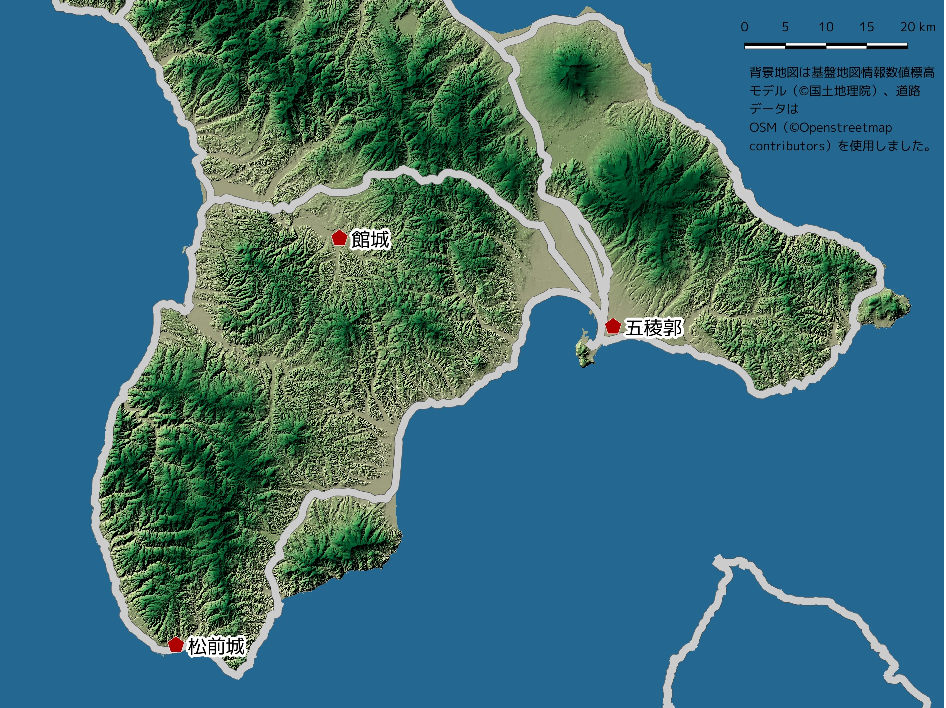
\includegraphics[width=160truemm]{fig/01map.pdf}
\caption{幕末期道南の城郭遺跡}
\label{fig01}
\end{figure}

%%%%%
\section{松前城の立地}
松前城は安政元年(1854)にそれまであった「福山館」を増改築する形で築城されました。松前は中世館跡の松前大館があり、中世から道南の拠点的な地域だったと考えられています\footnote{
中世の道南には「三守護職体制」と呼ばれる支配体制が存在し、「上ノ国」、「松前」、「下ノ国」の3地域のうち、「松前守護職」が特に中心的な権力であったと推測されています(海保嶺夫,1987)。松前氏の出自は上ノ国花沢館にいた蠣崎氏とされ、蠣崎氏は15世紀後半に勝山館を築きここを拠点としますが、永正11年(1514)の蠣崎光広のときに松前へ拠点を移します。それ以後、蠣崎・松前氏は松前を本拠地として勢力を確立していきます。
}
。
松前は北海道の最南端に位置し、津軽海峡に面しています。初期松前氏の財政基盤は、海産物、鷲羽、木材、砂金などの蝦夷地産物の輸出です。こうした蝦夷地産物の輸出と本州産物(米や酒、繊維製品)の蝦夷地への輸入による交易利潤が中世以来の道南勢力の財政基盤でした。松前藩は、こうした中世以来の財政基盤を幕藩体制に組み込んで制度化\footnote{
松前藩初代藩主松前慶広が徳川幕府から発給を受けた「黒印状」には蝦夷地と本州を結ぶ交易統制権が松前藩にあることを安堵した内容となっており、松前藩の蝦夷地支配の本質が交易統制権を根拠とした交易利潤にあったことをあらわしています。
}
することで、蝦夷地と本州の交易を統制することを藩の「生業」としてきました。松前城も、こうした松前藩の財政基盤に必要な機能を果たすために、海に面した立地が選ばれたものと考えられます。

%%%%%
\section{館城の立地}
一方、館城は厚沢部川の中流域、海岸線から厚沢部川沿いに約20kmさかのぼった厚沢部川左岸に立地しています。糠野川と厚沢部川に囲まれた台地上で厚沢部川本流が流れる館地区の平野部がよくみえる場所に位置しています。海を見下ろすように築城た松前城とは全く異なる立地です。

\begin{figure}[h]
\centering
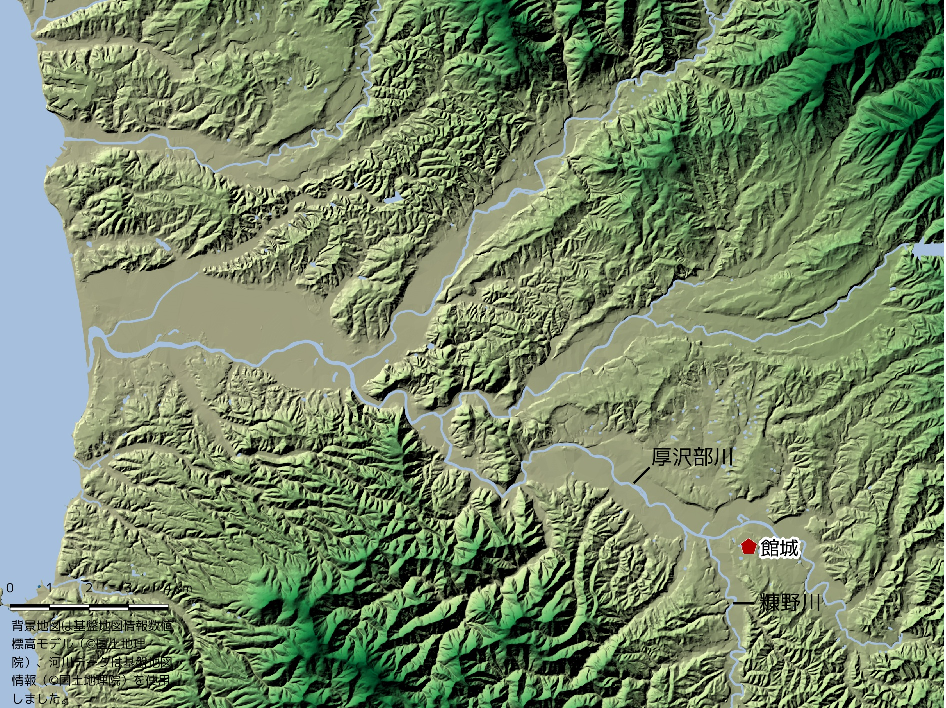
\includegraphics[width=160truemm]{fig/02map.pdf}
\caption{内陸に位置する館城}
\label{fig02}
\end{figure}

%%%%
\section{築城願書にみる館城}
館城築城に際して松前藩が提出した築城願書\footnote{
「厚沢部之内館エ御築城被成度御直願書」(北海道大学附属図書館北方資料室所蔵)は11月7日に提出された館城の築城願書です。11月7日はすでに築城工事が開始され、藩主徳広も入城していた時期です。新政府側について旧幕府方と交戦状態にあったため、書面と実態の齟齬についても黙認があったと考えられます。
}
では築城理由を次のように説明しています。

\begin{itemize}
\item 松前はかつては防衛に優れた地形と考えられてきたが、近年では大きな戦闘艦が来航し、松前城も危険にされされるようになった。
\item 厚沢部の館村は川と山に囲まれた天然の要害である。
\item 拓地勧農も将来は進むことが見込まれる。
\item 箱田奉行所へも陸路で近く、箱館で万が一のことがあれば、すぐに駆けつけることができる。
\end{itemize}

すなわち、内陸に立地することで大きな戦艦の砲撃を受ける危険が少なく、広い平野があるために農業開発にも適しており、開港地の箱館への交通も便利であると述べています。


%%%%
\newpage
\section{水田と厚沢部}
\begin{wrapfigure}{r}{15zw}
\vspace*{-\intextsep} 
\centering
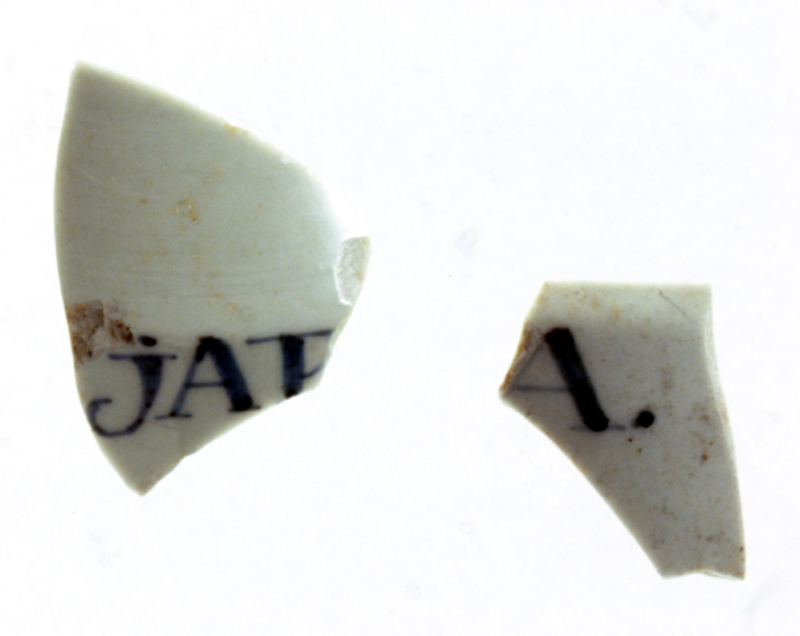
\includegraphics[width=15zw]{fig/11comp.png}
\caption{開墾役所跡から採取されたコンプラ瓶}
\label{fig11comp}
\end{wrapfigure}

近年、松前藩が安政年間頃(1860頃)から厚沢部川流域で本格的な水田開発を行っていた資料が発見されています。江差町郷土資料館所蔵の「脇家文書-038」の中に松前藩が越後からの農民の受け入れを行うための旅費の規定や農具貸付の規定などを整備していた記録が見つかっています。また、以前から厚沢部町字新栄に松前藩が設置した「開墾役所」\footnote{
松前藩が設置した開墾役所跡は館城から北西に直線距離で約3km離れた厚沢部川右岸の段丘上にあったとされています。館地区に開拓入植した二木小児郎の自伝『福寿草』に「下館の原野には米倉掘立柱の余燼数十基あり」とされ、開墾役所の痕跡を目撃した記録が知られています。昭和43年の農地開拓のパイロット事業工事で削平され、遺構の多くは消失したと考えられます。工事の際の地表面採集資料としてコンプラ瓶破片2点(図\ref{fig11comp})が採取されています。
}
があったと伝えられています。

松前藩領内の水田適地を傾斜にもとづいて算出したところ、主要な河川流域の中でも厚沢部川流域が特に大きな面積をもっていることがわかります(図\ref{fig03})。築城願書において松前藩が述べた「拓地勧農」は、現実に即した内容だったことがうかがえます。

\begin{figure}[h]
\centering
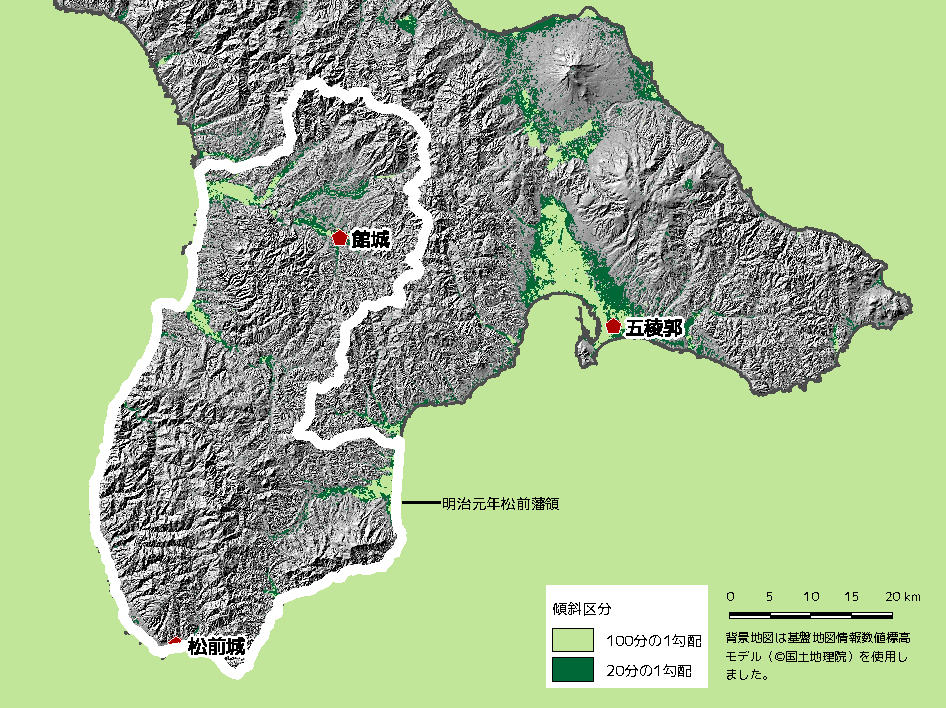
\includegraphics[width=160truemm]{fig/04slope.pdf}
\caption{広い平野をもつ厚沢部川流域}
\label{fig04}
\end{figure}

\begin{figure}[h]
\centering
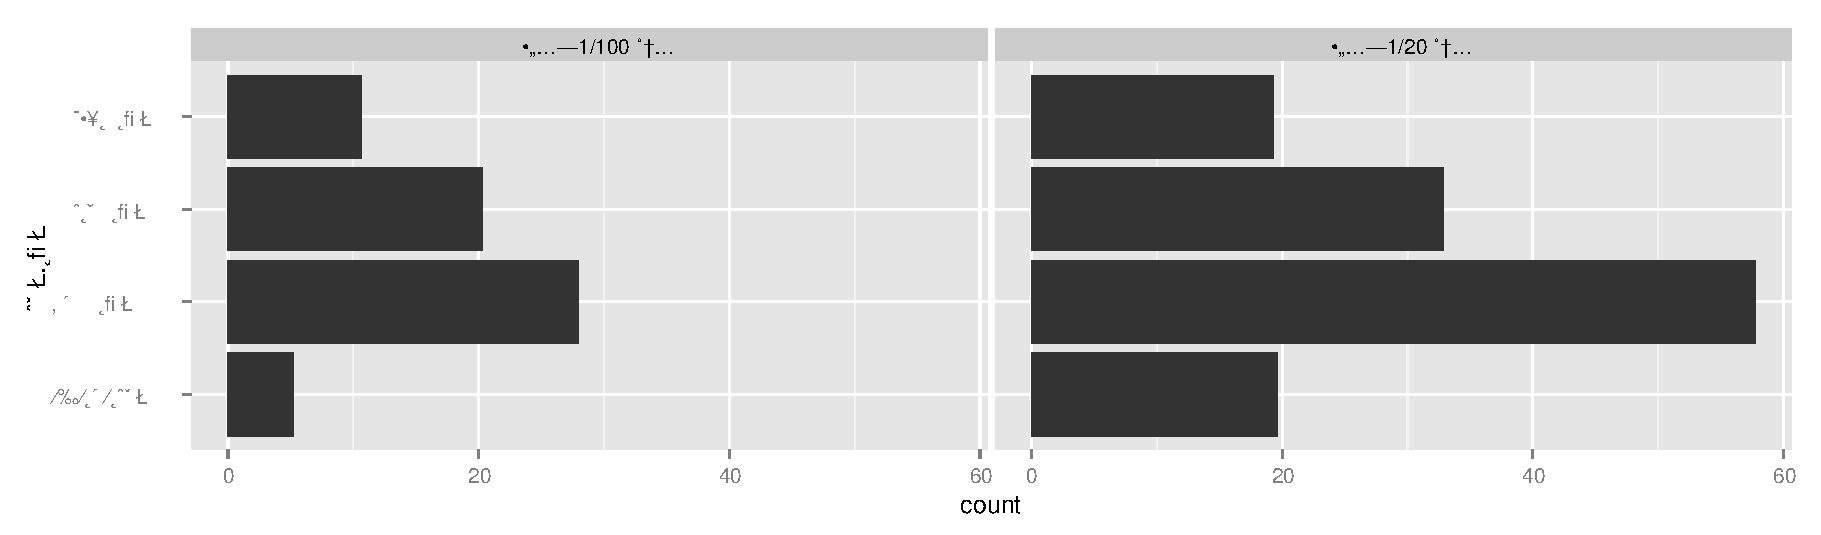
\includegraphics[width=160truemm]{fig/03suiden.pdf}
\caption{水田適地の多い厚沢部川}
\label{fig03}
\end{figure}

%%%%%
\newpage
\chapter{館城の築城と幕末の松前藩}
\section{近世の蝦夷地はどんな場所だったのか}
井上勝生(2002)は、18世紀後半から19世紀の幕末にいたる近世後期の日本社会を突き動かした原動力一つを「経済の上昇」にもとめています。これを支えた要因のひとつに「アイヌ民族と和人雇い漁夫が蝦夷地で生産したニシンの魚肥」があったといいます。井上によると農業生産増大にニシン肥があったことは当時に知識人にも認識されていたそうです。

近世後期の蝦夷地の流通は、文化文政期(1804〜1829)以降、いちじるしい上昇をみせます(榎森,1973)。このような漁獲物をはじめとする蝦夷地物産からの関税収入を松前藩では藩の経営基盤としていました。海保嶺夫(1986)によると、幕藩体制的蝦夷地支配の基本は以下のようなものだったと言われています。

\begin{itemize}
\item 松前城下を中心に、蝦夷地と本州の人や物の流通を統制すること
\item 蝦夷地への物資供給を松前藩士に限定すること
\item このことによって関税(沖之口)収入を財政基盤とすること
\item 同時に蝦夷地に住む人びとを事実上支配していること
\end{itemize}

%%%%%
\section{第2次蝦夷地幕領化}
以上のような幕藩体制的蝦夷地支配は、安政2年(1855)の第二次蝦夷地幕領化と安政6年(1859)の蝦夷地六藩分知によって転換を余儀なくされます。このとき、松前藩領内では松前藩士や松前領西在(現在の檜山管内)の住民による箱館奉行所や東北諸大名への嘆願が行われました(松前町史編集室1988,pp1160-1187)。

こうした状況下で松前藩は藩領内での水田開発に着手したと考えられます。先に紹介したように、厚沢部上流の館地区に開墾役所が設置されました。その結果、「江差周辺の村々や厚沢部、館、鶉などでは相応の田地が開拓された」という状況になっていたようです\footnote{
『御触書扣書』(松前町史編集室1974,pp)は知内村に出された触れ書きで、「江差周辺や厚沢部、館村、鶉村では田地の開発が進んでいる」ことから「知内村でも開発を進めるように」という内容となっています。「江差在々並びに厚沢部・館・宇津良」では「相応之田地相成」、「東西知内村広野之義も御取ひらき被成候旨仰出」
}
。

第二次幕領化によって、蝦夷地への流通統制権を事実上失った松前藩は、それまでの財政基盤である関税収入(沖之口役)が大幅に低下したため、農業開発による藩財政の再構築をめざしたものと考えられます。厚沢部の館地区には開墾役所が設置され、厚沢部川流域が松前藩領内でもっとも農業開発が進展していた様子がうかがえます。こうしたことから、松前藩領内において厚沢部川流域、特に館地区の重要性が高まっていたと考えられます。『工藤丹下長善履歴書』(永田1966)には千軒岳の麓を通って館村へ行く道路の開削の目的として、非常の際に館村に築城予定の城郭に密かに通行するためのものであることを、文久3年頃(1863)下国弾正から内密で漏らされた、とする記述\footnote{
『工藤丹下長善履歴書』には、館村への「営柵」の築造と館村への秘密の道路について次のように記載されています。「千間麓より館村広野に至るの間道開鑿」の目的は非常の際に「館広野」に建設予定の「営柵」へ、「山手密行」するためである。この部分は原文確認
}
があり、館城築城以前に館地区へ城郭の建設計画が密かに持ち上がっていたことをうかがわせます。



%%%%%
\section{13代藩主崇広の死去と徳広の藩主就任}
松前藩13代藩主松前崇広は、慶応2年四月に病死します『北門史綱』巻六,永田1991)。祟広は1万石格の外様大名としては異例の昇進をとげ、元治元年(1864)には老中格海陸総奉行の地位となります。この頃、祟広の行動は自ずと江戸を中心としたものとなり、国元の政治は松前勘解由などの家老を中心に行われることとなりました。このことが、後に藩主の世継ぎ問題をはらんだ内紛へとつながります。

崇広の死後、12代藩主の嫡子徳広が藩主に就任するものの、病弱な徳広は政務を執ることができず、藩政の中枢は、松前勘解由など崇広時代の重臣らが掌握したままでした。こうした状況に反発する反勘解由派の藩士達が、『建言書』(『慶応二丙寅十一月旧寄合中より建言書』 江差町史編集室1979,pp)を藩主徳広に上申しました。これにより松前勘解由は家老職を辞すこととなりますが、反勘解由派の蠣崎民部らは脱
藩の罪に問われ、また、藩政は依然として勘解由派が取りしきっていました。

%%%%%
\section{正議隊のクーデター}
明治元(1868)年7月28日、反勘解由派の藩士達は、『正議隊建白書』(江差町史編集室1979,pp465-468)を藩主徳広に提出しました。『建白書』を受けた徳広は、勘解由ほか4名の重臣の登城を差し止めましたが、勘解由らはこれにしたがわず、町役所に諸士を呼び集め密議を行なったといいます(『奉命日誌』江差町史編集室1979,pp429-463)。

7月29日、江差奉行尾見雄三が、江差在郷藩士らを率いて江差から出動し、8月1日に福山城下へ到着しました(『慶応四年四月より行事見聞録』江差町史編集室1983,pp8-13)。尾見は、かねてから江差在郷の藩士や江差商人団を反勘解由派に引き込んでいたことから、江差商人団が反勘解由派の資金源となったとの見解もあります(江差町史編集委員会1983,p5)が、江差商人関川与一の残した『慶応四年四月より行事見聞録』(江差町史編集委員会1983,pp8-13)\footnote{
関川与市の『慶応四年四月より行事見聞録』には次の記載があります。「一、七月廿九日晴 夕七ツ時ニ候哉御役所半鐘打出し候故、市中半鐘打合 何事ニやと聞会候処 詰木石出火又ハ津花町出火之よし 実説不相分夫是致し候内 石崎村へ蒸気舟至来 バッテラニ而人数三十人 或三百人上陸 同所ニおゐて乱防致し近々当方へ馳向候様子(中略)右之大変後日承り候処 全蒸気舟来着抔ハ尾身雄三謀斗ニ而 人数繰出し為に有之よし」。外国船が上ノ国石崎村へ来航し、三百人が上陸し乱暴を働いているため、尾見雄三率いる江差市中の藩士が出動したということになっていましたが、これは松前の正義隊と合流するための出陣をカムフラージュするための謀略だったことが後に明らかになったということです。
}
や藤枝日記の「慶応四年七月二十九日」(江差町史編集委員会1979,p1479)の記事
では、尾見らの松前出陣については全く情報がなくうろたえる様子が示されているので、江差商人団と正義隊の関わりを陰謀論的に捉えることは難しいと考えられます。

尾見の到着により勢力を増した正議隊は、8月1日から勘解由派の粛清を開始しました。一連の粛清は、9月24日の山下雄城の処刑をもって一段落し、勘解由派の主要人物のほとんどを殺害する結果となっりました。

%%%%
\section{館城の築城}
館城築城工事の経過は、勘定奉行兼作事方を任命された江差の豪商、関川重孝(平四郎)が残した日記(江差町史編集室1981,pp1220-1301)によって知ることができます。関川平四郎の日記から館城築城工事の様子は次のとおりです。

9月2日に館村の鈴木文五郎に宛てて遠眼鏡を送ったことが記されており、この時期に、担当者が現地入りしていたことを知ることができます。9月14日には、大工四十人・木挽十人が館へ向けて出立している。9月21日には、福山から大工棟梁孝次郎はじめ、下職28名が江差へ到着し、館へ向けて出立しました。また、9月12日頃から土木作業が開始されており、9月23日現在の延べ人工数は、1,525人工に達しています。

9月28日現在の館城普請に係る人員は、大工棟梁浜田仁兵衛、幸治郎以下、大工小頭五人、木挽2人、平大工92人、下木挽21人、土方小頭7人、土方243人、人足183人となっています。

10月14日には、建具師3人が木材と供に館へ向かっており、また、10月16日には、間似合、唐紙、玉子などの襖材料が館へ送られており、館城普請は、内装作業へと移りつつあったことがわかります。
10月24日には、棟上げの儀式が行われたことが記されており、城内の重要な建物の棟上げが行われたと考えられます。

10月26日には、森町鷲ノ木に上陸し、箱館をめざして進軍中の旧幕府軍と新政府軍との交戦が七飯峠下で行われたことを受けて三上超
順や今井興之丞\footnote{
三上超順と今井興之丞はいずれも館城攻防戦で戦死した松前藩の武将です。両者はこの方面における松前藩軍の軍事的な指導者だったと考えられます。
}
が、手勢を引き連れて木間内まで出張しています。館城普請の最終的な結果について、日記には触れられていませんが、関川重孝の築城日記もこの10月26日をもって終わっていることから、この前後に、館城の普請もほぼ終了していたと考えられます。

%%%%%
\newpage
\chapter{館城の守りの工夫を知る}
\section{館城は「陣屋のような城」なのか}
同縮尺で松前城と館城を比較した図\ref{fig05}から、館城跡と福山城跡の規模がほぼ同じであることがわかります。館城の築城コンセプトについては、「館城が新造なった福山城の本丸御殿を縮小コピーしたような施設だった」(姫路市立城郭研究室2006)との見解もありますが、平面規模からみる限り、館城は松前城(福山城)本丸御殿の「縮小コピー」ではなく、松前城と同規模の城郭を新築しようとしたものということができます。また、平成14年の館城跡追加指定説明として「その構えは城郭というより陣屋に近」いとされていますが\footnote{
城郭用語に「陣屋」という用語はありません。当時の人びとが「陣屋」と呼んだり「台場」と呼んだりした歴史的経緯に配慮して「陣屋」、「台場」などを固有名称として使用することがありますが、城郭の構造を形容する場合において「陣屋のような」という表現はナンセンスです。
}
、松前藩が館城築城に際して意図したものは簡易な軍事施設ではなく、本拠地松前城に代わる新しい藩の居城だったと理解するべきです。

\begin{figure}[h]
\centering
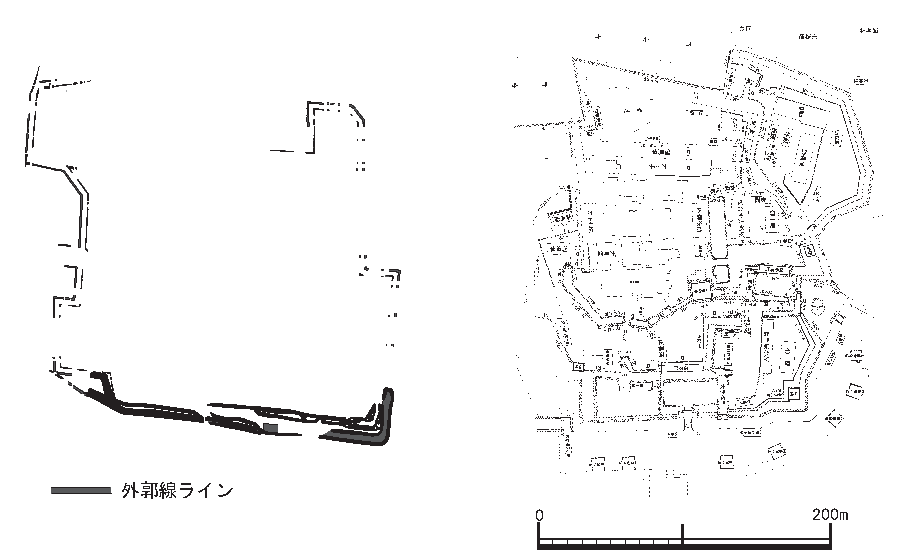
\includegraphics[width=160truemm]{fig/05.pdf}
\caption{館城と松前城は同じ大きさ}
\label{fig05}
\end{figure}

%%%%%
\section{出入り口の工夫を知る}
館城へ入るためには、西側、あるいは北側から接近するのが一般的です。江差方面、函館方面いずれから館城を目指すとしても必ず、館の平野を通って館城へ向かうこととなります。館城の正面出入り口は西側に設けられました(図\ref{fig06})。

\begin{figure}[h]
\centering
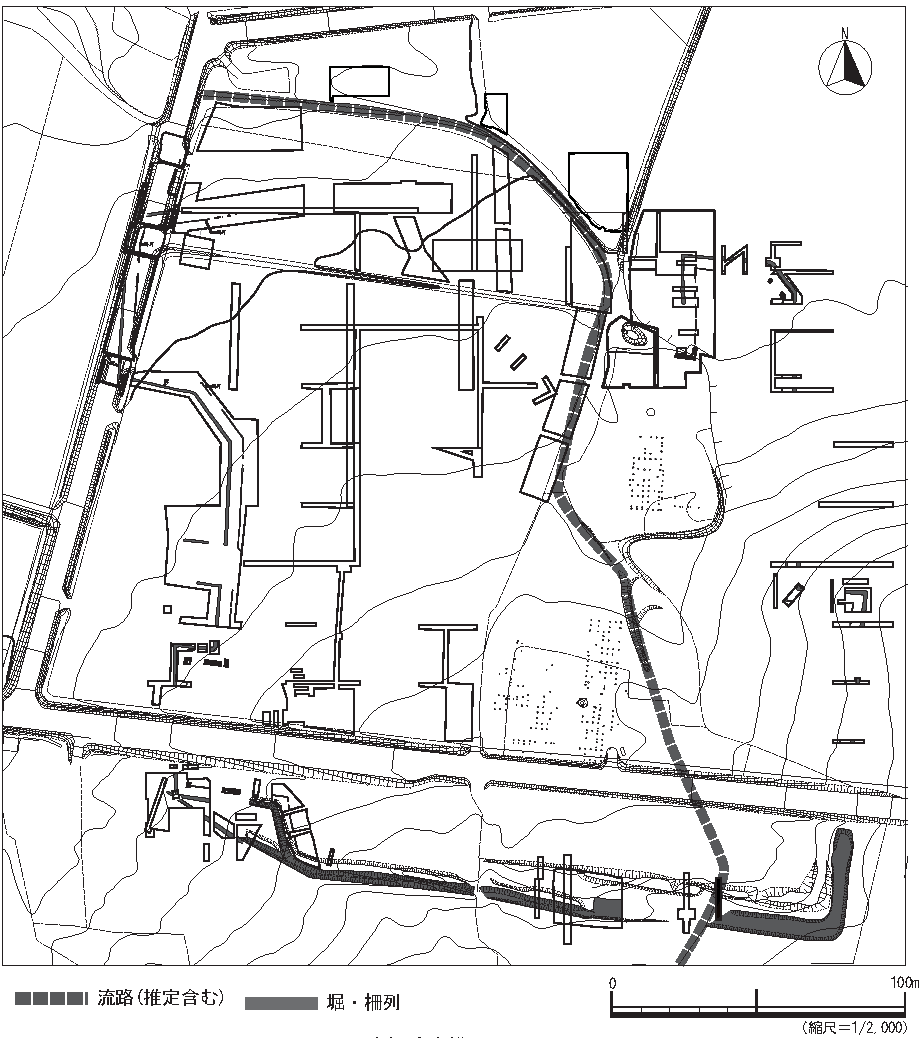
\includegraphics[width=160truemm]{fig/06.pdf}
\caption{館城は西側が正面}
\label{fig06}
\end{figure}

館城の出入り口は、両脇の塁線が大きく城外に張り出した「両袖型」といわれる構造です(図\ref{fig07})。出入り口部分が城内に引っ込んだようになっているため、出入り口に近づいた敵は、大きく城外に張り出した塁線の守備兵から十字砲火を受けることになります。この構造が館城の出入り口の大きな特徴です。同じような構造が松前城の搦手出入り口にも採用されています。

また、出入り口に10m四方ほどの区画を設けて外側に張り出させています。これは「外枡形」あるいは「外馬出し」と呼ばれる構造かもしれません。「枡形」や「馬出し」は防禦の際には敵を誘い込んで集中攻撃を浴びせかける仕組みであると同時に、いよいよ反撃する場合には兵を待機させておく出撃拠点ともなるものです。遺構の残り具合が悪くはっきりしたことはいえませんが、松前城の正面出入り口にも外馬出しが設けられていますので、館城にもそのような工夫がされていた可能性を考えています。

\begin{figure}[h]
\centering
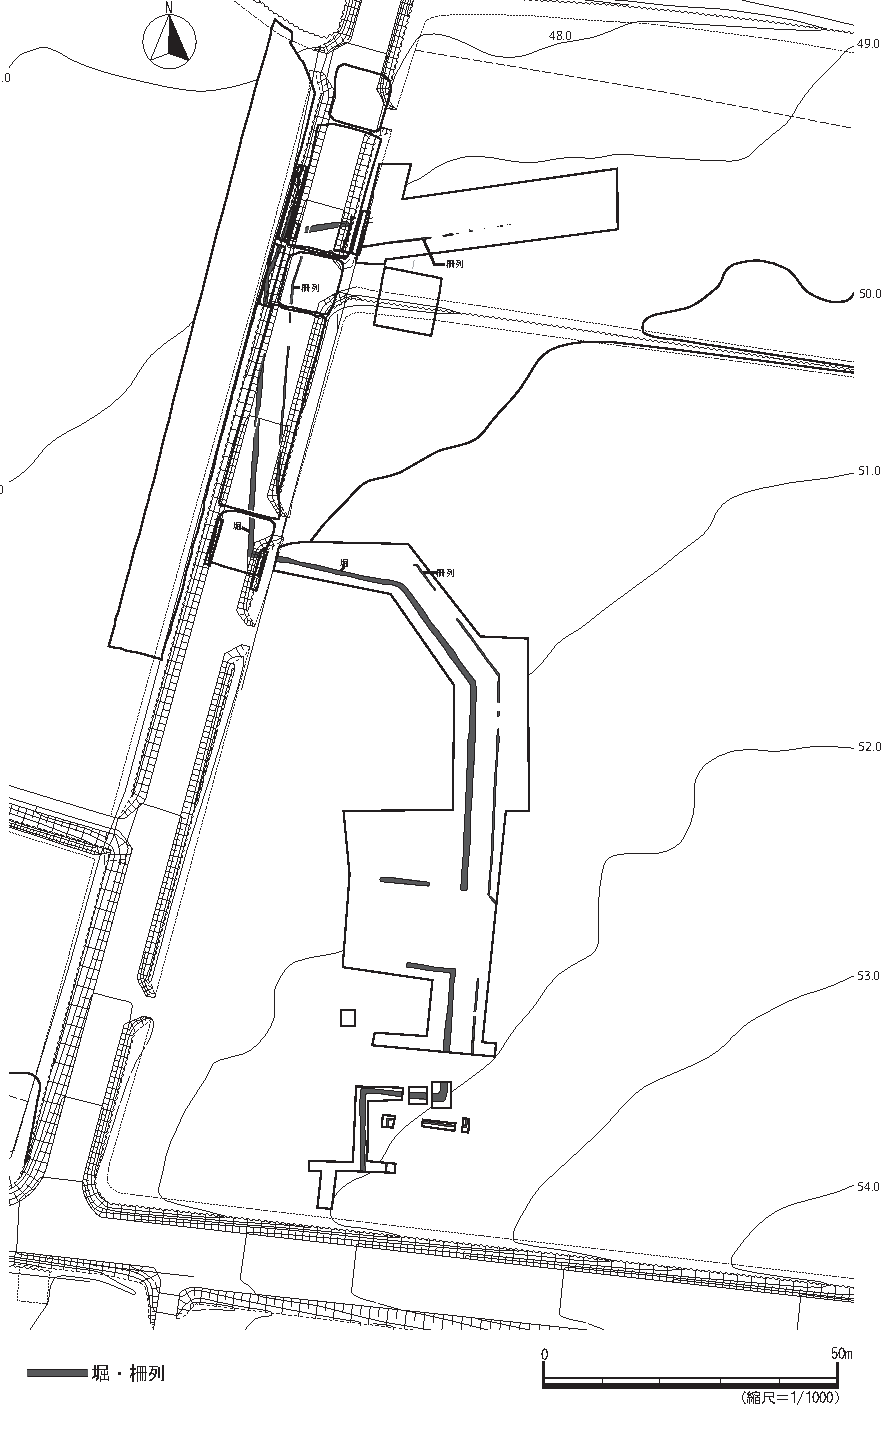
\includegraphics[height=230truemm]{fig/07.pdf}
\caption{「両袖型」の館城出入り口}
\label{fig07}
\end{figure}

%%%%%
\section{災いを防ぐ鬼門除け}
館城北東部には現実的な守りの工夫だけではなく、霊的な守りの工夫もみられます。図\ref{fig08}に示すように、北東部のコーナーは直角ではなく45度に切り落とされています。これは「鬼門」にあたる北東方向を出隅にせず角を落としたものです。藩主の居城として、あらゆる面で抜かりなく備えていたことがわかります。

\begin{figure}[h]
\centering
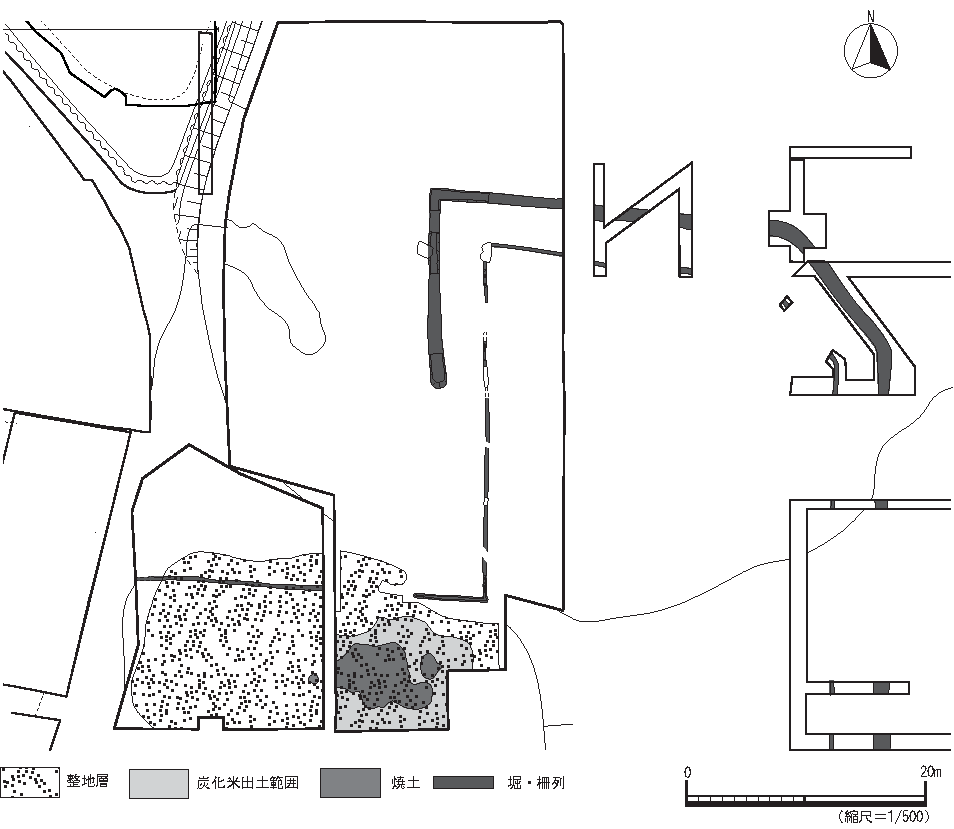
\includegraphics[width=160truemm]{fig/08.pdf}
\caption{北東隅の「鬼門除け」}
\label{fig08}
\end{figure}

%%%%%
\section{守りの要となる柵}
館城の守りは堀、土塁、柵で構成されています。外側から堀→土塁→柵という順に防御施設が設けられ、敵を防ぐ仕組みになっています。柵は土塁の内側、堀の中心から約4.2mのところに位置します。

柵は「布掘り」という手法でつくられています。「布掘り」とは、柵を立てるラインに溝を掘っておき、溝の中に柵柱を立てて溝を埋め戻す方法です。手間がかからないことと、予定のラインを維持しやすいことが利点です(図\ref{fig09})。

柵柱の深さは確認された面から0.6mありました。実際には10cmほど掘り下げているので、実際の埋め込まれた深さはもう少し深かったと考えられます。このくらいの深さでは、横板を貼って板塀のようにした場合、控柱などがないと風などに耐えることができないと考えられます。ところが、これまでの発掘調査で控柱と考えられる痕跡は全く発見されていません。したがって、館城の柵は単なる柱列で、せいぜい柱を連結するための横木(貫のような構造も考えられる)があったものと考えられます。

『松前沖之口奉行所図』\footnote{
『松前沖之口奉行所図』は、第一次蝦夷地幕領化(1799~1821)に伴い沖之口奉行所となった松前城(福山館)の外観を描いた写生図です。国立公文書館所蔵
}
(以下「奉行所図」)に描かれた松前城(福山館)北東部の柵列を図\ref{fig10}に示しました。また、同縮尺で館城の柵の推定模式図を掲載しました。『奉行所図』に描かれる松前城の柵列は、館城跡の柵列の木柱と比較して一周り太い角材が使用されています。柱間距離の正確な計測はできませんが、0.2〜0.3m程度と読み取れそうです。木柱の上部をヌキで連結する構造で、控柱などは確認できません。柵の高さは前景の人物から比較計測すると雪面から約1.3mです。積雪深を0.5mと推測すると無雪期の柵列地表高は1.8mとなります。俯瞰の影響や前景人物との遠近法的技法の影響は考慮していませんが、おおむね以上のような寸法だったと考えられます。

館城の柵は、近世城郭の守りの施設としてはいかにも脆弱ですが、改築前の松前城(福山館)の絵図と比べると館城で検出された柵とよく似た構造のすき間だらけの柵が描かれていますので、不自然ではないと考えています。

\begin{figure}[h]
\centering
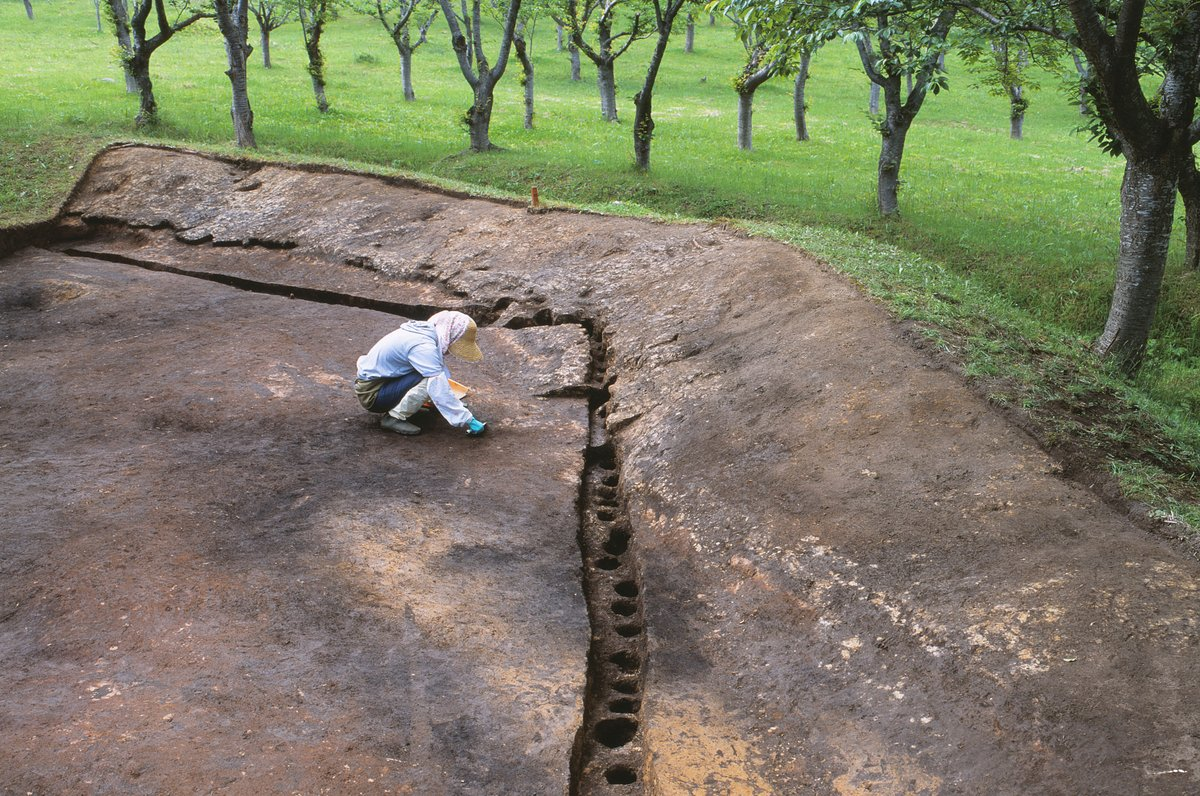
\includegraphics[width=160truemm]{fig/09.JPG}
\caption{発掘された館城の柵}
\label{fig09}
\end{figure}

\begin{figure}[h]
\centering
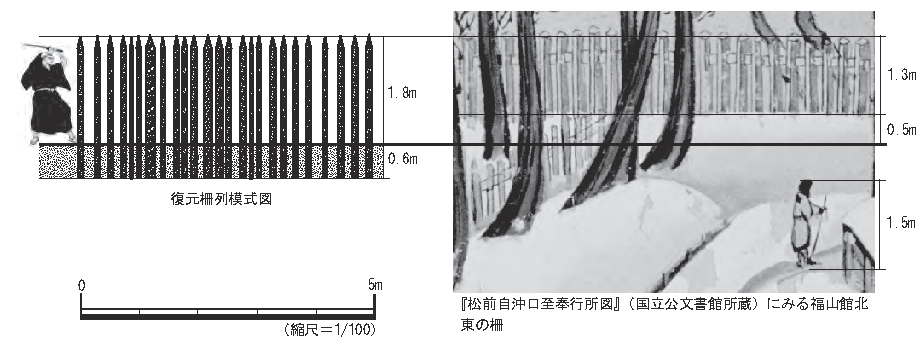
\includegraphics[width=160truemm]{fig/10.pdf}
\caption{松前藩の伝統、すき間だらけの柵}
\label{fig10}
\end{figure}

%%%%%%
\newpage
\chapter{お殿様の建物}
\section{地面をつついて建物をさがす}
\begin{wrapfigure}{r}{15zw}
\vspace*{-\intextsep} 
\centering
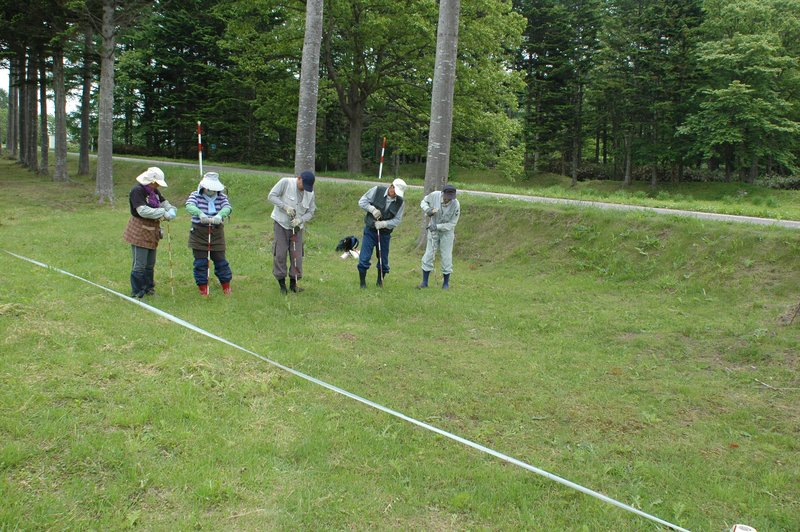
\includegraphics[width=15zw]{fig/14.JPG}
\caption{みんなで並んで建物を探す}
\label{fig14}
\end{wrapfigure}

平成21年に館城の建物の痕跡(礎石)をさがすための調査を実施しました。掘削を行わず地面をピンポールでつついて礎石を探しました。
図\ref{fig11}にはしっかりと礎石が残っていた場所だけを図面に記していますが、抜き取られた礎石も多く、図面に示した礎石は、当初あったもののごく一部であると判断しています。

\begin{figure}[h]
\centering
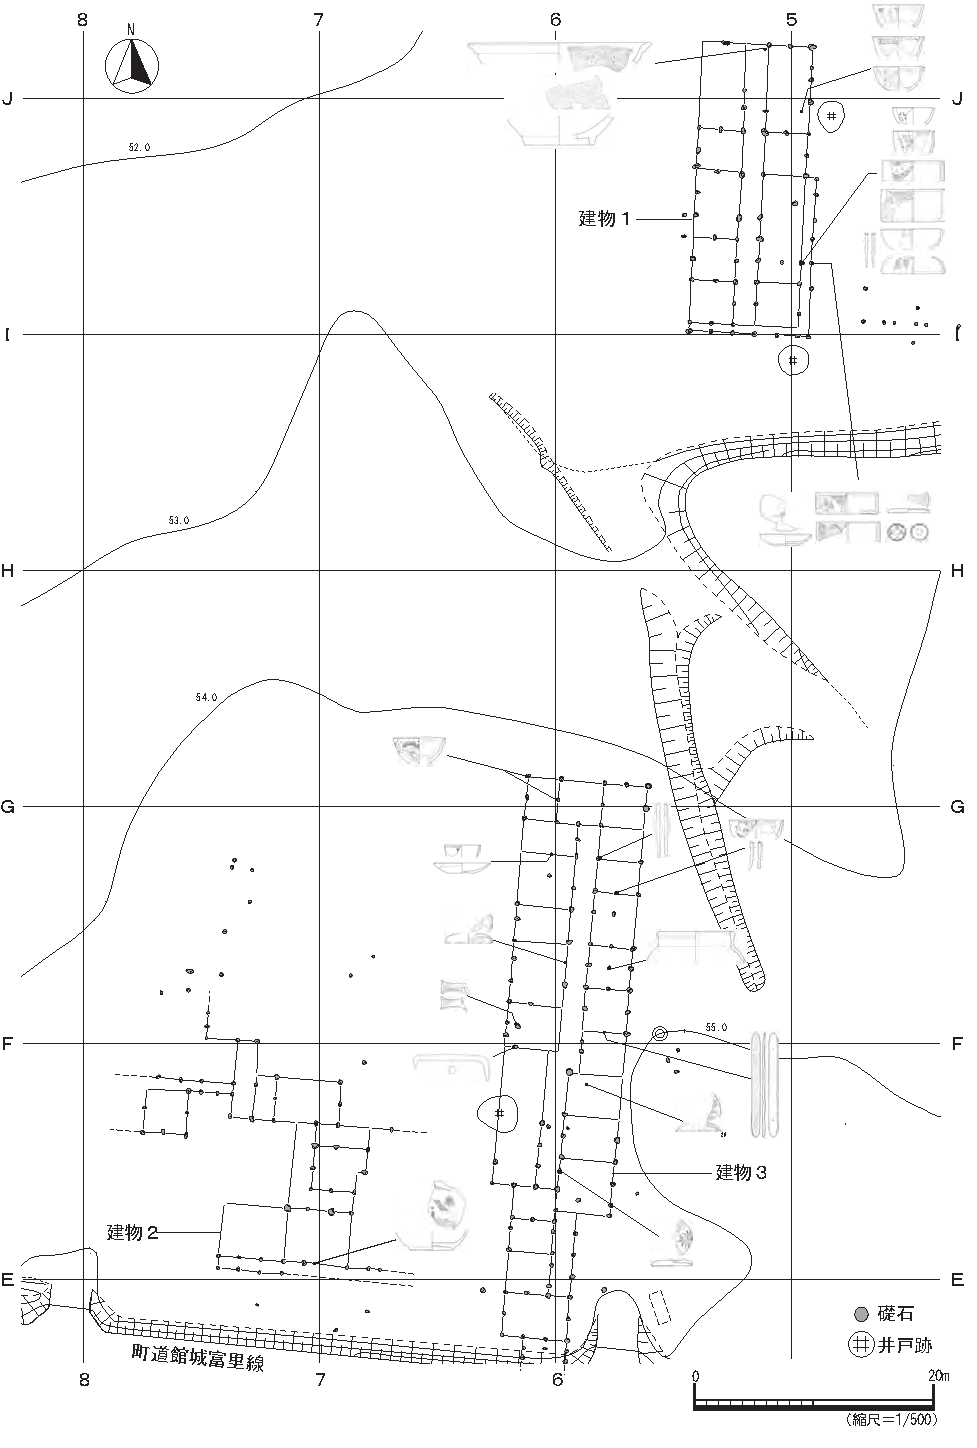
\includegraphics[width=150truemm]{fig/11.pdf}
\caption{発見された館城の建物}
\label{fig11}
\end{figure}

\section{どんな建物があったのか}
\begin{wrapfigure}{r}{15zw}
\vspace*{-\intextsep} 
\centering
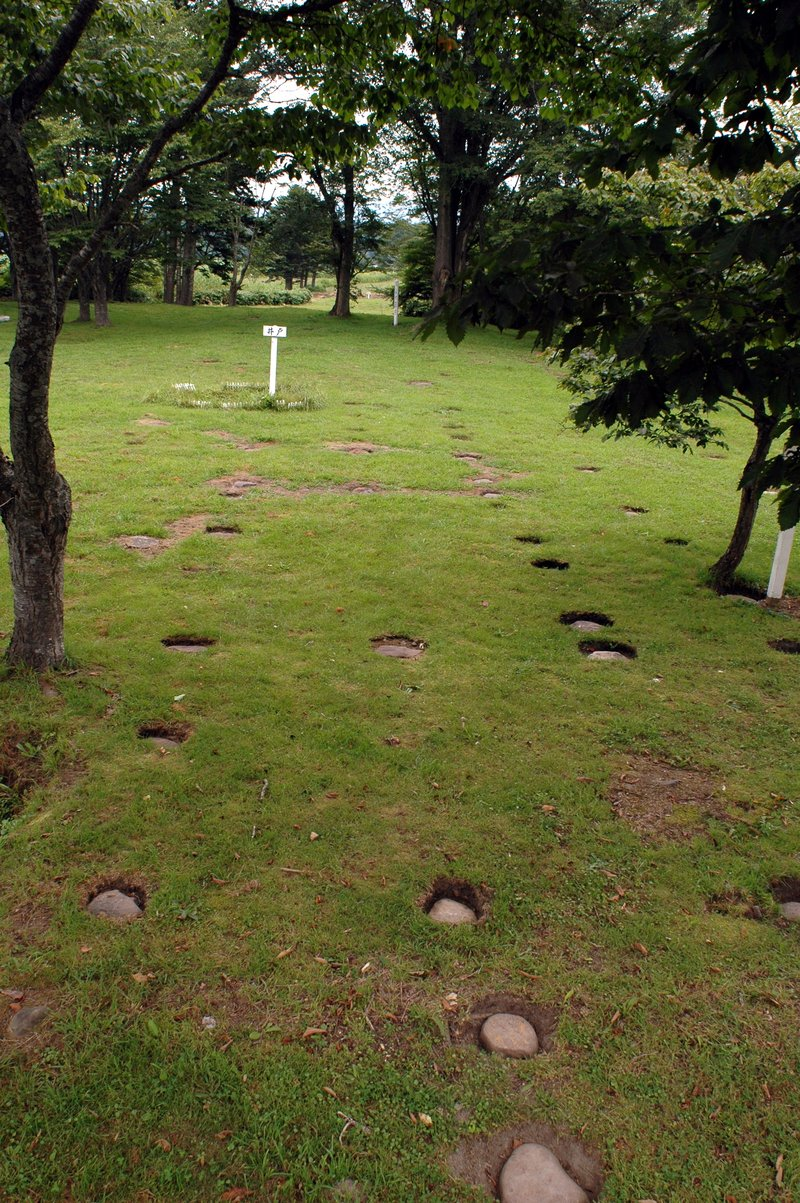
\includegraphics[width=15zw]{fig/15.JPG}
\caption{みつかった建物の礎石}
\label{fig15}
\end{wrapfigure}

合計3棟の建物が見つかりました。町道館城富里線の北側に並ぶ2棟と沢を挟んで北側に1棟の建物がみつかりました。

「建物1」は、梁行5間、桁行 13 間で中央に廊下が通ります。廊下の左右に部屋が設けられています。建物3の南面と東面には「縁」が附属します。碗類や段重などの食膳具、すり鉢が採取されました。段重がまとまって採取された点が特徴です。

「建物2」(図\ref{fig12}左側)は未検出の礎石が多く、全体の構造は不明で。「コの字」又は回廊状の平面と考えられます。出土遺物が陶磁器皿1点のみとなっていることが、多くの遺物が見つかった建物1と異なっています。

「建物3」(図\ref{fig11}右側)は、梁行5間半、桁行 27 間の細長い建物です。桁行方向の南側は町道が上をおおっているので、南の端は確認できませんでした。建物1は、中央に廊下が通り、左右に部屋が設けられる構造です。南側では廊下が途切れ、4つの部屋が連続して配置されています。礎石のまわりから、お碗や急須などの陶磁器類、屏風の平金具、釘、かすがいなどの建築部材がみつかっています。

%%%%%
\section{増田家文書『館築城圖』とくらべる}
図\ref{fig12}の『館築城圖』は、増田家文書\footnote{
増田家文書の筆者である増田伝左衞門幹通は、幕末から明治前期にかけて江差沖之口役所内下代、会計局権督事、湊司、国産司、足軽頭、土木司、算数方を兼務し、松前藩政期末の藩吏を務めたとされます(江差町史編集室,1977)。本図面を増田幹通が所蔵することとなった経緯は不明です。
}
として知られる資料群に含まれる絵図で厚沢部町教育委員会が作成した写本です。館城に築かれた御殿の平面図と考えています。後述するように、現地の礎石配置と一致点も多いのですが、決定的に異なる部分もあることから採用されなかった設計図と考えています。

\begin{figure}[h]
\centering
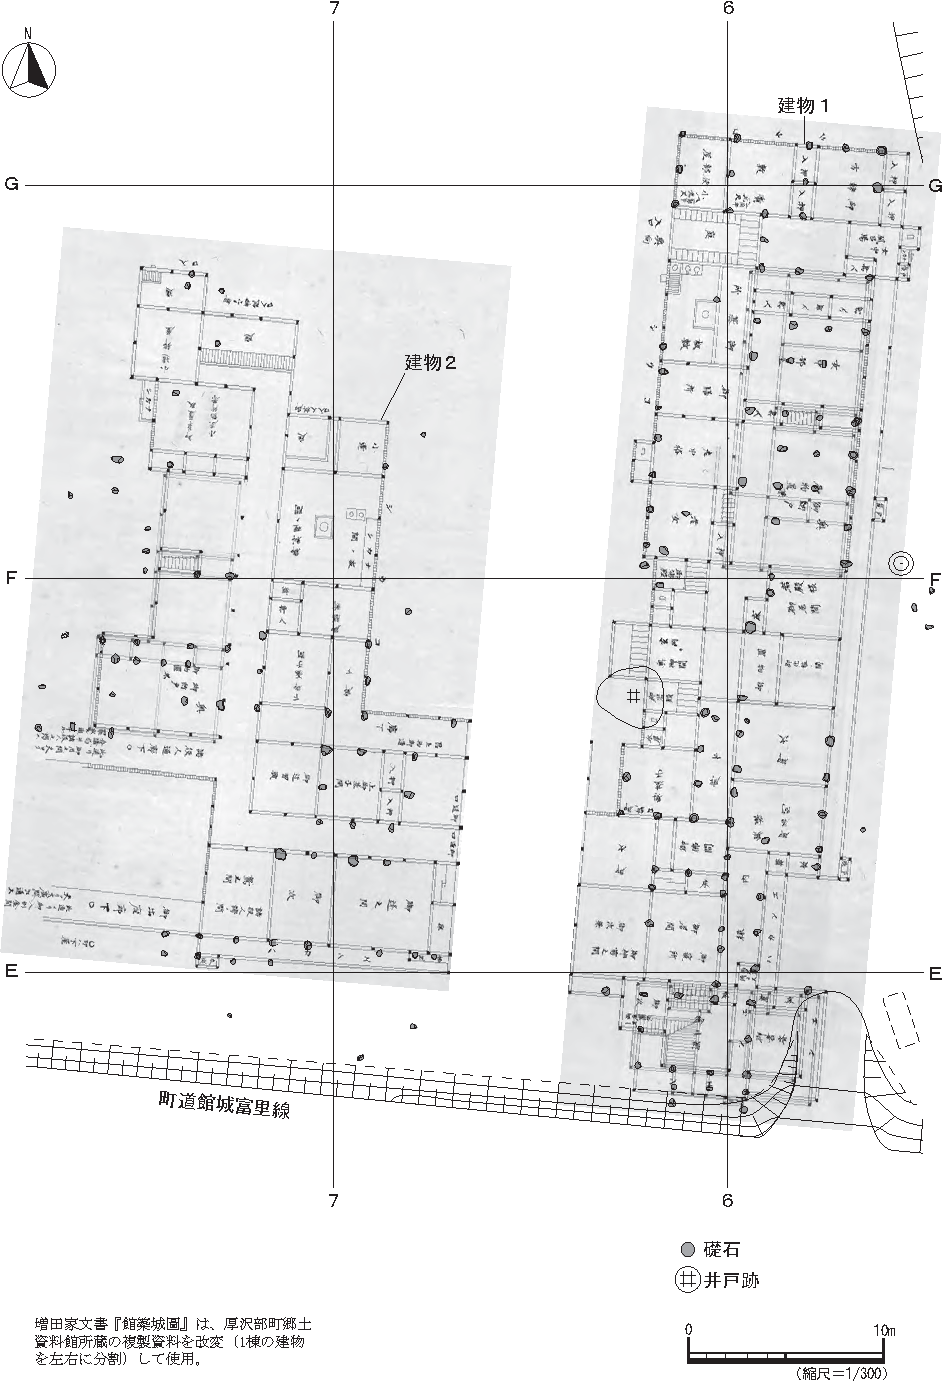
\includegraphics[width=160truemm]{fig/12.pdf}
\caption{増田家文書『館築城圖』と見つかった礎石}
\label{fig12}
\end{figure}


図\ref{fig12}の現地の礎石配置と『館築城圖』を重ね合わせる際には、『館築城圖』で1棟として描かれた建物を二つに切り分けてます。『館地築城圖』では、現地で検出された「建物2」と「建物3」を合わせたような「L字」の大きな1棟の建物が描かれています。しかし、現地の礎石配置は少なくとも8m以上礎石が検出されない区間があることから、「建物2」と「建物3」は別の建物であったことは間違いありません。『館築城圖』と現地の礎石を重ね合わせるためには、『館築城圖』を2つに切り分けるしかありませんでした。

『館築城圖』右半の建物(建物3)の南側には「御寝所御居間」、「奥様御居間」、「若殿様御居間」などの注記がみられ、北側には「老女」、
「女中部屋」、「御臺所」(図中は「御基所」と誤記)などの注記が見られます。つまり、「建物3」は藩主家族とその身廻りの世話をする女性たちが詰める「奥御殿」に相当する建物だったことがわかりました。

『館築城圖』左半の建物(建物2)は南東部に床や棚が設けられた書院風の「御逢之間」や「諸役人謁ノ間」、「上御臺子」、「下御臺子」(図中は「基子」と誤記)、
「御料理ノ間」などがみられます。これらの部屋は藩主の日中の居所とそれに伴う部屋で、藩主が政務を行い、家臣との面会などを行う「常御殿」に相当する建物だったことがわかりました。

さらに、「御出座廊下」、「諸役人通廊下」などの注記があることから、図の左側(現地では西側)にもう1棟、別の建物があったことがうかがえます。「御出座廊下」には「此の通ヨリ御入例金間夫ヨリ大廣間江通ス」との注記が付されており、「諸役人通廊下」には、「此通リ御用之間夫ヨリ合議局並諸役人之謁ニ罷出ル通ニナル」との注記が付されています。つまり、『館築城圖』左半の建物(建物2)のさらに左は次のような構造になっていたと考えられます。

\begin{itemize}
\item 「御出座廊下」の先には「金間」と呼ばれる部屋があり、その先に「大廣間」がある。
\item 「諸役人通廊下」の先には「御用之間」があり、その先に「合議局」がある。
\end{itemize}

以上のことから、『館築城圖』にかかれていない左側の建物は、公式な対面や藩士らが政務を行う「表御殿」に相当する建物であったと推測できます。

%%%%%
\section{福山館本丸御殿の間取と比較する}
図\ref{fig13}は「松前自沖口至奉行所図」所収の『松前奉行所経営地割図』\footnote{
『松前奉行所経営地割図』は第一次蝦夷地幕領化(1799〜1821)に伴い沖之口奉行所となった福山館の全体平面図です。安政元年(1854)
の福山城改修以前の姿を知ることができる資料です。
}
(以下『地割図』)です。

\begin{figure}[h]
\centering
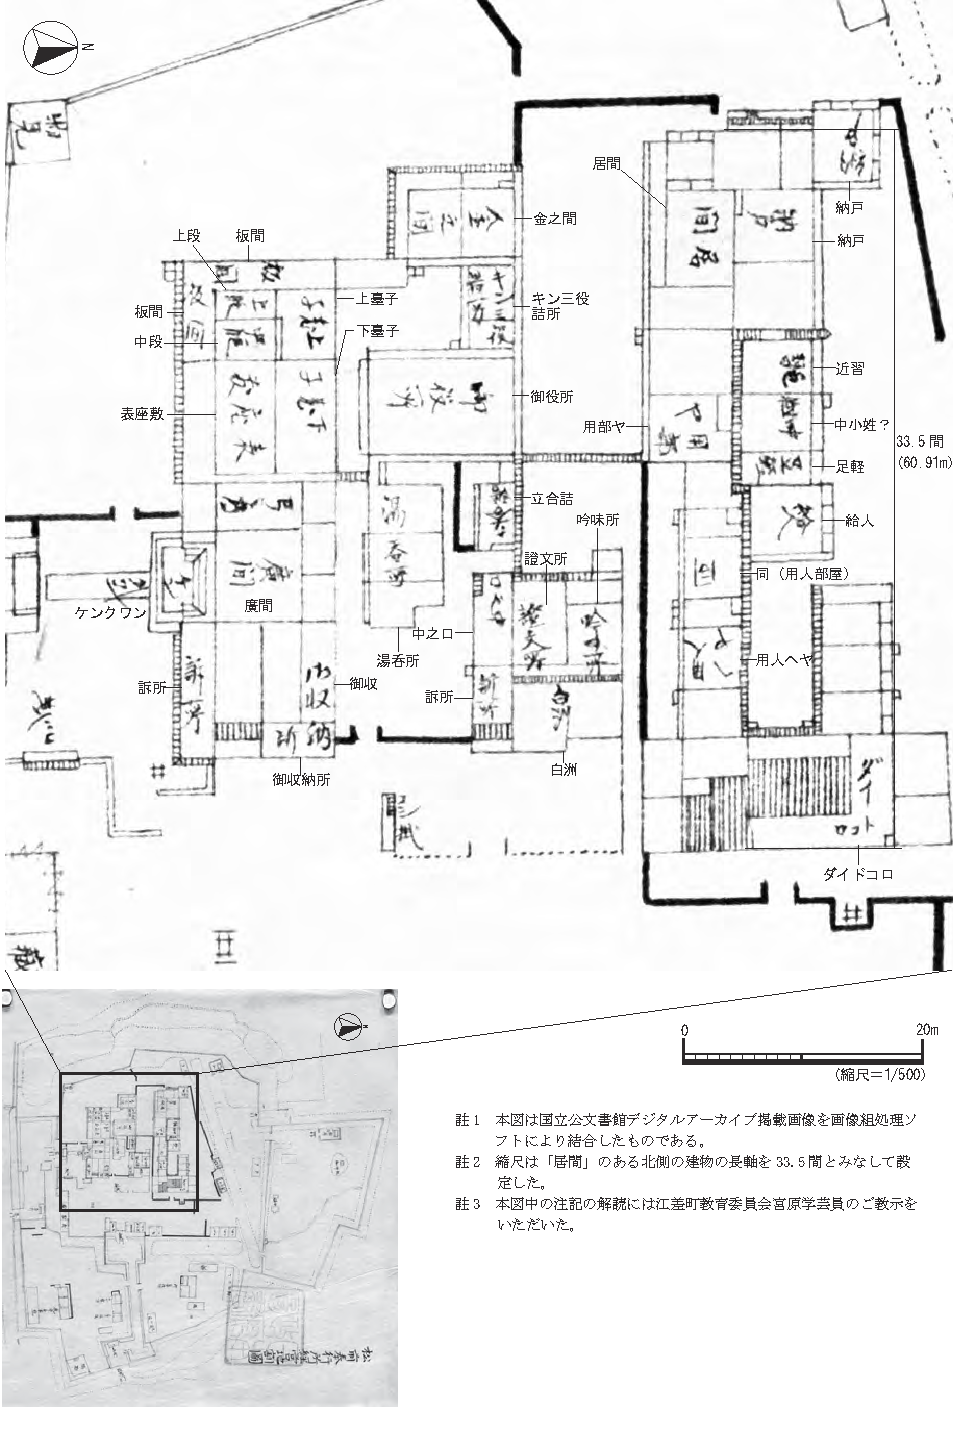
\includegraphics[width=160truemm]{fig/13.pdf}
\caption{福山館本丸御殿(「松前奉行所経営地割圖」(『松前自沖口至奉行所図』所収(国立公文書館所蔵))に加筆)}
\label{fig13}
\end{figure}

「金之間」、「上下臺子」、「廣間」は『館築城圖』の「金間」、「上(下)御臺子間」、「大廣間」にそれぞれ一致します。「地割図」に描かれた福山館本丸御殿の右半(北側)の建物は奥御殿に相当する建物で、左半(南側)の建物は常御殿と表御殿を兼ねた建物と考えられます。
「コの字」形に配された建物群の中央には「吟味所」、「訴所」、「白洲」など裁判所の機能をもった建物が描かれます。
『館築城圖』が示す館城の御殿に比べると、常御殿、表御殿の部分が一棟にまとめられており、施設の機能分化が未熟だったようです。


%%%%%
\section{松前城本丸御殿の間取と比較する}
『渡嶋国津軽郡福山旧城内建物』\footnote{
北海道庁所蔵の開拓使簿書「官舎倉庫其他官舎絵図表明治九年十二月函館支庁」に所収
}
(以下『旧城内建物』)では、4連棟の本丸御殿が描かれます。安政元年に完成した松前城では、福山館時代の城郭を拡張し、砲座をもつ三の丸の築造をはじめ、大改修が行われました。松前藩の政治・行政の中心となる本丸御殿についても大きく様変わりしています。

『旧松城小学校解体事業調査報告書』(遠藤ほか1984)では「本丸御殿の建築年は不明」とされ、「安政元年の福山城築城工事の際の記録には、この表御殿の造営には言及していないから、この際には建築工事が行われなかったことは確実である」と述べられています。本丸御殿の築造年代については「福山秘府年歴部巻之四や新羅之記録下巻がつたえる寛永 14 年(1637- 筆者註)3 月 28 日夜の火災で焼失した後に、再建した建物ということになる」とされいていますが、『旧城内建物』の本丸御殿図と『地割図』の建物は明らかに異なっていることから、福山館の御殿は文化年間以降に改築されたことは明らかです。文化年間の『地割図』に描かれた機能分化が未熟な2連棟の御殿が福山館時代の御殿の姿であり、その後、改築時期は不明ながら、4連棟の御殿が築造されたと考えるのが自然です。

館城では4連棟の御殿の構造を引継ぎながら、3連棟の御殿が計画されたと考えられます。


%%%%
\newpage
\chapter{出土遺物から考える館城}
\section{陣屋や漁場と比べる}
館城の特徴は、出土した陶磁器の構成を他の遺跡との比較すると明らかになります。比較対象とした遺跡は、北海道内で19世紀代を中心に営まれた白老町白老仙台藩陣屋跡、根室市穂香川右岸遺跡、苫小牧市弁天貝塚、別海町野付通行屋跡の4遺跡です\footnote{
函館市五稜郭跡や松前町福山城跡、北斗市戸切地陣屋跡など幕府関係や松前藩関係遺跡との比較も興味深い作業ですが、陶磁器構成比が明らかにされていないため比較対象としていません。今後の研究課題の一つです。
}
。

%%%%
\section{お皿が多い館城}
館城では、碗・皿類の比率が6割を超えていることが特徴的です。 特に皿類の構成比率が突出しています。館城出土の皿は、他の遺跡で多く出土する輪花皿(三平皿)に加えて、大型の皿類が多く出土しています。館城以外の遺跡では相対的に壺・甕・瓶の比率が高く、穂香川右岸遺跡や、弁天貝塚、野付通行屋跡では出土量の6割以上をこれらが占めています。弁天貝塚や穂香川右岸遺跡では特に越後産の瓶(焼酎徳利)の出土量が多く、壺・甕・瓶の比率の高さにつながったと考えられます。

%%%%
\section{陣屋や漁場とは明らかに異なる陶磁器の構成}

\begin{wrapfigure}{r}{80truemm}
\vspace*{-\intextsep} 
\centering
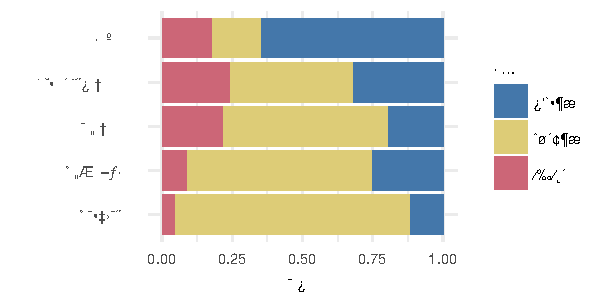
\includegraphics[width=80truemm]{fig/16.pdf}
\caption{食膳具の多い館城}
\label{fig16}
\end{wrapfigure}

遺跡の性格別にみると、館城跡は藩主の居所、白老仙台藩陣屋跡は北方警備のための軍事拠点と警衛地の経営、穂香川右岸遺跡と弁天貝塚は漁場関係、野付通行屋跡は人馬継立などを行う交通の拠点です。このうち、穂香川右岸遺跡や弁天貝塚は松前藩や幕府などの権力との関わりが最も薄く、次いで幕府によって設立された野付通行屋跡、仙台藩が藩士を送り込み軍事・行政の拠点とした白老仙台藩陣屋跡は権力の関与が高いと考えられます。館城跡は、松前藩の新たな拠点として築造されたことから、これらの遺跡群の中では最も権力との関わりが強い遺跡といえます。
このような遺跡の性格の違いを踏まえると、館城跡の陶磁器構成比の特徴は以下のように整理できます。

\begin{enumerate}
\item 碗 ・ 皿類などの食膳具の高い構成比率は、陶磁器を用いる食事を頻繁に大人数で行う環境を示して
おり、公的な食事の機会の多い藩の拠点としての性格を示しています。
\item 特に皿類の構成比率が高いことは、多人数の食事に用いられる大型の皿類が多いことを示し、儀礼
的な食事=宴席機会の多さが想定されます。
\item 壺 ・ 甕 ・ 瓶類の出土比率の少なさは、存続期間の短い館城では日常雑器であるこれらの器種の廃棄
数量が少なかったことと、下層階級で好まれた焼酎の消費量が少なかったことを意味します。
\item 陣屋跡や漁場関係遺跡などと比較して館城跡の陶磁器構成比は特徴的であり、その特徴は藩主の居
所と藩の拠点としての遺跡の性格に直結していると考えられます。
\end{enumerate}


%%%%
\chapter{館城は完成していたのか}
\section{完成していなかった証拠}
『報功心血』\footnote{
著者は元松前藩士の今井微。原本は所在不明で、函館市中央図書館所蔵の写本のみが確認される。写本は、昭和2年の図書館公立化に際して私立時代の蔵書から引き継いだものである(函館市中央図書館田村昌弘氏の教示による)。明治26年以後の成立と考えられる。
}
によると館城の築城については春をまって堀の外側の工事を行う予定であったこと\footnote{
「濠外の如きは觧雪の期を待つ修築すへきの予想なりき」(『報功心血』)
}
、戦闘の備えは不十分であったこと
\footnote{
「有事の警備に至ては、未た其配置を效すへきの余力なきのみならす、この短時日の能く為す所にあらす」(『報功心血』)
}
が示されています。

築城開始から工事終了まで2ヶ月足らずの短期間であることを考えると堀の外側に予定されていた外構や防御のための設備については不十分だったと考えることは妥当です。

%%%%
\section{完成していた御殿}
一方、『報功心血』によると以下のような施設があったとされています
\footnote{
『報功心血』には次のように記されています。「ニ大廈を経営して、外部は空濠を環らし、濠頭に径尺の丸木を併列して、僅かに牙城の形勢を規模し、西北に二門を以て稍塁砦の一片を成せり。」
}
。

\begin{itemize}
\item 大きな二つの建物
\item 空堀
\item 丸木の柵
\item 西と北に門
\end{itemize}

このうち、空堀や柵は発掘調査でその存在が確認されており、西側の門についても門の遺構は確認されていませんが、西側に正面と思われる出入り口があることは確認されています。「大きな二つの建物」については、礎石を検出した「建物2」や「建物3」がこれに該当する可能性がありそうです。

%%%%
\section{紅皿が語るもの}

\begin{wrapfigure}{r}{40truemm}
\vspace*{-\intextsep} 
\centering
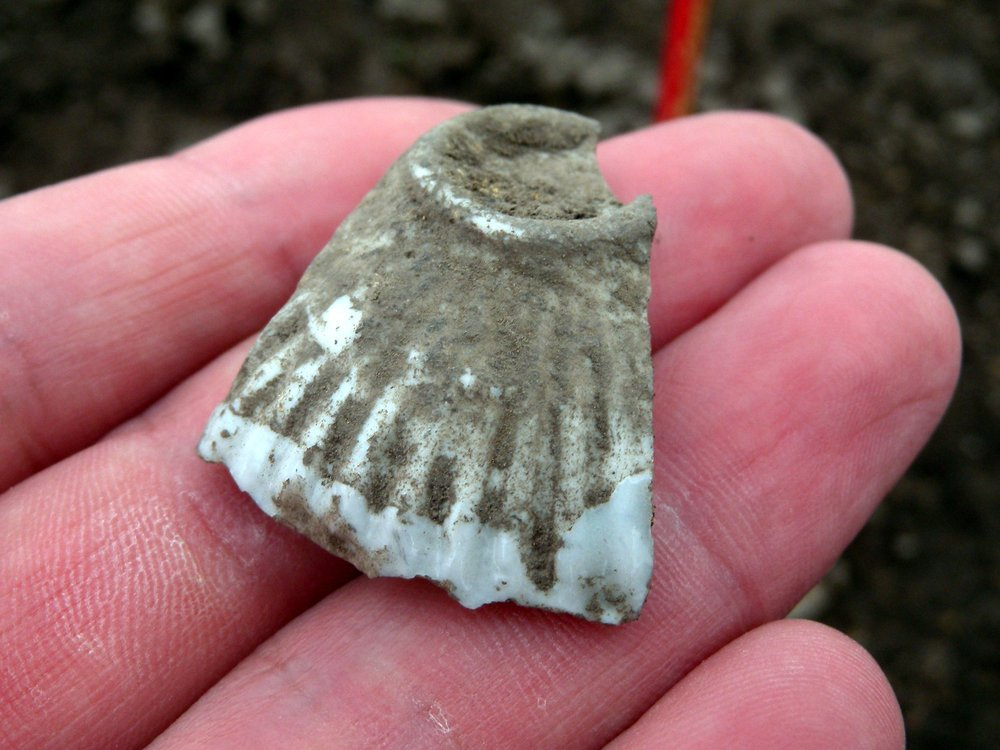
\includegraphics[width=40truemm]{fig/17.JPG}
\caption{館城に身分の高い女性がいた証拠「紅皿」}
\label{fig17}
\end{wrapfigure}

館城では「\ruby{紅皿}{べにざら}」が出土しています。「紅皿」とは女性の化粧道具です。館城で見つかったものは、飾り気のない白い釉薬がかけられたものです。館城出土の多くの陶磁器は松前藩が備品として準備したものです。しかし、「紅皿」は個人所有物と考えられます。つまり、館城から出土した「紅皿」は、それを所有した女性本人が館城にいた証拠です。

「紅」をさすような女性とは、藩主やその家族の身の回りの世話をする「お女中」や「老女」などが考えられます。そのような女性がすでに館城内にいたということは、藩主を迎え入れるための建築がある程度完成していた可能性が高いことを意味します。

%%%%
\section{屏風を野ざらしにはしないはず}

\begin{wrapfigure}{r}{25truemm}
\vspace*{-\intextsep} 
\centering
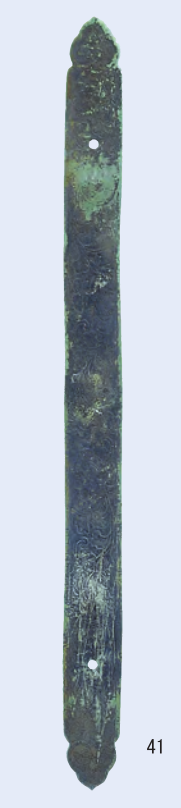
\includegraphics[width=15truemm]{fig/18.png}
\caption{屏風につけられていた金具}
\label{fig18}
\end{wrapfigure}

もう一つ、館城からは屏風の側面につけられた平金具が出土しています。屏風はかさばるもので、水に弱いものです。こうした調度品が館城に搬入されていたことは、屏風などを使うような格式の高い建物がすでに館城に存在したことを意味します。館城から多くの陶磁器が出土していることとあわせて考えると、館城には屏風や高価なひと揃いの食器が搬入されており、これらを必要とする建物が存在したことがわかります。

%%%%
\section{館城、完成・未完成論争の決着}
『報功心血』が述べるように、館城全体としてはまだまだ未完成な部分が多く、松前版では翌春に工事を再開する見通しがあったことがわかります。一方、館城内部にはすでに屏風や食器が搬入されるとともに、紅をさすような女性がいた可能性が高いことがわかっています。

つまり、全体として未完成ながらも、一部については高い完成度をもっていたと考えられます。松前藩は藩主を迎えるための建築工事を急ぎ行い、堀や土塁、柵を含めた外構については後回しにした可能性があります。もともと戦争のための施設として建設されたのではなく、松前藩の新しい拠点として館城が築城されたと考えると、こうした工事の優先順位にも納得がいくものです。


%%%%
\chapter{館城のもつ意味}
\section{松前藩の新たな拠点}
\begin{itemize}
\item 内陸深くに立地する館城は、海沿いに立地する松前城とは異なる機能をもつ城郭です。
\item これは、蝦夷地産物の輸出入から、農業経営へと藩の経済基盤を変質させることが目的でした。
\item そのため、館城は水田適地である厚沢部川の中流に築城されました。
\end{itemize}

%%%%
\section{陣屋とはまったく異なる構造の館城}
\begin{itemize}
\item 松前藩が意図したものは、松前城にかわる新しい藩の拠点でした。
\item 「福山城本丸御殿を縮小コピーしたもの」でも「陣屋に近い」ものでもなくリニューアルされた松前城でした。
\item 館城の規模や出入り口の構造が松前城に酷似しているのは当然です。
\end{itemize}

%%%%
\section{藩の中心となる御殿の跡}
\begin{itemize}
\item 館城でみつかった礎石の配置は、『館築城圖』に記された御殿の平面図と一致点が多いものです。
\item 『館築城圖』に描かれた建物は「奥御殿」、「常御殿」に相当する建物で、さらに「表御殿」に相当する建物があったことが示唆されています。
\item 「金ノ間」や「台子ノ間」などは松前城の御殿に見られる特徴的な部屋です。
\item 以上のことから、館城で見つかった礎石は松前藩の御殿に相当する建物だったと考えられます。
\end{itemize}

%%%%
\section{館城の特徴を示す出土遺物}
\begin{itemize}
\item 館城の出土遺物は食膳具が多く含まれています。
\item 陣屋や漁場遺跡と比較した際に、その特徴は際立っています。
\item 藩主の居城であり、松前藩の新たな中心地として築かれた館城の特徴がよく示されています。
\item 出土遺物からみても館城は「陣屋に近い」城郭ではありませんでした。
\end{itemize}

%%%%
\section{近世的な蝦夷地の終わり}
館城の築城は、近世的な蝦夷地の終わりを示すものです。松前藩は、蝦夷地と本州の交易を統制することを藩の経営基盤としてきました。このような経済構造・支配構造が「近世的な蝦夷地」の本質です。海上交通の統制に便利の良い松前から、内陸で水田適地への本拠地の移動は、松前藩が、交易統制を行うことを事実上断念したことを意味します。

近代の北海道は、これまで「外国(異域)」として扱われてきた北海道が内国化・植民地化の対象となっていく時代です。館城の築城は、幕藩体制的蝦夷地の終焉と近代北海道の始まりを象徴するできごとと評価したいと思います。


%%%%%
\newpage
\chapter{参考文献}
\mbox{}\\
井上勝生 2002「序章 人間の静かな大地」『開国と幕末変革』日本の歴史18,講談社,pp7-23\\
江差町史編集室 1979『江差町史』第3巻資料3,江差町\\
江差町史編集室 1981『江差町史』第4巻資料4(関川家文書)江差町\\
江差町史編集室 1983『江差町史』第6巻通説2,江差町\\
榎森進 1974「報告4 近世北海道の流通構造」『松前藩と松前ー松前町史研究紀要ー』4号,松前町史編集室,pp37-54\\
遠藤明久編 1984『旧松城小学校解体事業調査報告書』松前町\\
海保峰夫 1987「第五 中世蝦夷地の変容」『中世の蝦夷地』吉川弘文館,pp208-253	\\
永田富智 1966「工藤丹下長善履歴書(ニ)」『新しい道史』4巻6号,pp\\
永田富智 1991「北門史綱(前承-巻之四より巻之七)」『松前藩と松前ー松前町史研究紀要ー』33号,松前町史編集室,pp1-100\\
姫路市立城郭研究室 2006「戦争中に築かれた城」『姫路市立城郭研究室ニュース 城踏』No.64\\
二木小児郎 1937『福寿草 二木小児郎自叙伝』(厚沢部町教育研究会社会科サークル 2003年発行復刻版)\\
松崎岩穂 1973『続上ノ国町史』上ノ国村\\
松前町史編集室 1974『松前町史資料編』第1巻\\
松前町史編集室 1988「松前町史通説編」第1巻下\\



\end{document}  
